%%%%%%%%%%%%%%%%%%%%%%%%%%%%%%%%%%%%%%%%%%%%%%%%%%%%%%%%
% chapters/ese1.tex
%%%%%%%%%%%%%%%%%%%%%%%%%%%%%%%%%%%%%%%%%%%%%%%%%%%%%%%%
\chapter{Esercizio 1: Analisi di Segnali}

\section{Definizione della Trasformata di Fourier (FT)}

La Trasformata di Fourier (FT) di un segnale $x(t)$ è definita come:
\begin{equation*}
    X(f) = \mathcal{F}\{x(t)\} = \int_{-\infty}^{\infty} x(t) e^{-j2\pi f t} \,dt
\end{equation*}

L'Anti-trasformata di Fourier (IFT) di $X(f)$ è definita come:
\begin{equation*}
    x(t) = \mathcal{F}^{-1}\{X(f)\} = \int_{-\infty}^{\infty} X(f) e^{j2\pi f t} \,df
\end{equation*}

\section{Proprietà della Trasformata di Fourier}
Di seguito sono riassunte le principali proprietà della Trasformata di Fourier in una tabella.

\begin{table}[h!]
\centering
\caption{Proprietà della Trasformata di Fourier.}
\label{tab:ft_properties}
\begin{tabular}{lll}
    \toprule
    \textbf{Proprietà} & \textbf{Dominio del Tempo} & \textbf{Dominio della Frequenza} \\
    \midrule
    Linearità & $a x(t) + b y(t)$ & $a X(f) + b Y(f)$ \\
    \addlinespace
    Traslazione nel Tempo & $x(t - t_0)$ & $X(f) e^{-j2\pi f t_0}$ \\
    \addlinespace
    Modulazione & $x(t) e^{j2\pi f_0 t}$ & $X(f - f_0)$ \\
    \addlinespace
    Convoluzione & $x(t) * y(t)$ & $X(f) \cdot Y(f)$ \\
    \addlinespace
    Moltiplicazione & $x(t) \cdot y(t)$ & $X(f) * Y(f)$ \\
    \addlinespace
    Dualità & $X(t)$ & $x(-f)$ \\
    \addlinespace
    Derivazione nel Tempo & $\dfrac{d^n x(t)}{dt^n}$ & $(j2\pi f)^n X(f)$ \\
    \bottomrule
\end{tabular}
\end{table}


\section{Relazioni di Eulero}
Le formule di Eulero sono fondamentali per scomporre segnali sinusoidali e cosinusoidali:
\begin{align*}
    \cos(\theta) &= \frac{e^{j\theta} + e^{-j\theta}}{2} \\
    \sin(\theta) &= \frac{e^{j\theta} - e^{-j\theta}}{2j}
\end{align*}
Queste permettono di applicare la proprietà di modulazione a segnali come $\cos(2\pi f_0 t)$ e $\sin(2\pi f_0 t)$.

\section{Teorema di Parseval (Energia del Segnale)}
L'energia $E_x$ di un segnale può essere calcolata sia nel dominio del tempo che della frequenza:
\begin{equation*}
    E_x = \int_{-\infty}^{\infty} |x(t)|^2 \,dt = \int_{-\infty}^{\infty} |X(f)|^2 \,df
\end{equation*}

\section{Coppie Notevoli di Trasformate di Fourier}

\begin{center}
\begin{tabular}{c c}
    \toprule
    \textbf{Segnale nel Tempo $x(t)$} & \textbf{Trasformata di Fourier $X(f)$} \\
    \midrule
    $\rect\left(\frac{t}{T}\right)$ & $T \sinc(fT)$ \\
    \addlinespace
    $T \sinc(tT)$ & $\rect\left(\frac{f}{T}\right)$ \\
    \addlinespace
    $\tri\left(\frac{t}{T}\right)$ & $T \sinc^2(fT)$ \\
    \addlinespace
    $T \sinc^2(tT)$ & $\tri\left(\frac{f}{T}\right)$ \\
    \addlinespace
    $\delta(t)$ & $1$ \\
    \addlinespace
    $1$ & $\delta(f)$ \\
    \addlinespace
    $e^{j2\pi f_0 t}$ & $\delta(f - f_0)$ \\
    \addlinespace
    $\cos(2\pi f_0 t)$ & $\frac{1}{2}\left[\delta(f - f_0) + \delta(f + f_0)\right]$ \\
    \addlinespace
    $\sin(2\pi f_0 t)$ & $\frac{1}{2j}\left[\delta(f - f_0) - \delta(f + f_0)\right]$ \\
    \addlinespace
    $e^{-at} u(t), \quad a>0$ & $\dfrac{1}{a + j2\pi f}$ \\
    \addlinespace
    $e^{-\pi t^2}$ (Gaussiana) & $e^{-\pi f^2}$ (Gaussiana) \\
    \bottomrule
\end{tabular}
\end{center}

\subsection*{Definizioni delle Funzioni Base}
\begin{itemize}
    \item \textbf{Funzione Rettangolo (rect):}
    \begin{equation*}
        \rect(t) = 
        \begin{cases} 
            1 & \text{per } |t| < 1/2 \\
            1/2 & \text{per } |t| = 1/2 \\
            0 & \text{altrove}
        \end{cases}
    \end{equation*}
    
    \begin{figure}[h!]
        \centering
        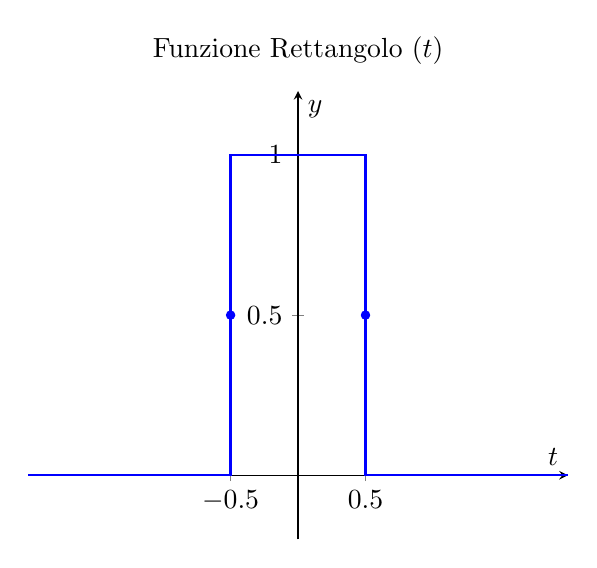
\begin{tikzpicture}
            \begin{axis}[
                axis lines=middle,
                xlabel=$t$,
                ylabel={$y$},
                title={Funzione Rettangolo $\rect(t)$},
                xmin=-2, xmax=2,
                ymin=-0.2, ymax=1.2,
                enlargelimits=false,
                ytick={0, 0.5, 1},
                xtick={-0.5, 0.5},
            ]
            \addplot[blue, thick, const plot] coordinates {(-2,0) (-0.5,0) (-0.5,1) (0.5,1) (0.5,0) (2,0)};
            \addplot[only marks, mark=*, blue, mark size=1.5pt] coordinates {(-0.5,0.5) (0.5,0.5)};
            \end{axis}
        \end{tikzpicture}
    \end{figure}
    
    \item \textbf{Funzione Seno Cardinale (sinc):}
    \begin{equation*}
        \sinc(t) = \frac{\sin(\pi t)}{\pi t}
    \end{equation*}

    \begin{figure}[h!]
        \centering
        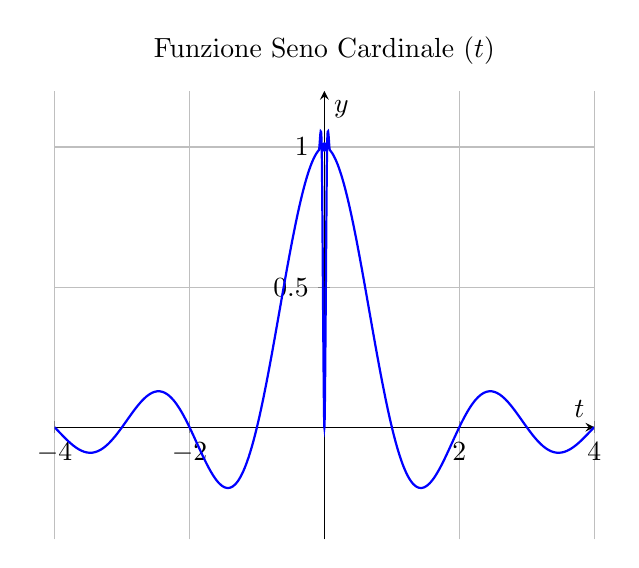
\begin{tikzpicture}
            \begin{axis}[
                axis lines=middle,
                xlabel=$t$,
                ylabel={$y$},
                title={Funzione Seno Cardinale $\sinc(t)$},
                xmin=-4, xmax=4,
                ymin=-0.4, ymax=1.2,
                enlargelimits=false,
                samples=201, % Aumenta i campioni per una curva liscia
                grid=major,
            ]
            \addplot[blue, thick, smooth, domain=-4:4] {sin(deg(pi*x))/(pi*x)};
            % Aggiunge un punto in (0,1) per gestire la singolarità
            \addplot[only marks, mark=*, blue, mark size=1.5pt] coordinates {(0,1)};
            \end{axis}
        \end{tikzpicture}
    \end{figure}

    \item \textbf{Funzione Triangolo (tri):}
    \begin{equation*}
        \tri(t) = 
        \begin{cases} 
            1 - |t| & \text{per } |t| < 1 \\
            0 & \text{altrove}
        \end{cases}
    \end{equation*}
    La funzione triangolo può anche essere vista come la convoluzione di due rettangoli: $\tri(t) = \rect(t) * \rect(t)$.

    \begin{figure}[h!]
        \centering
        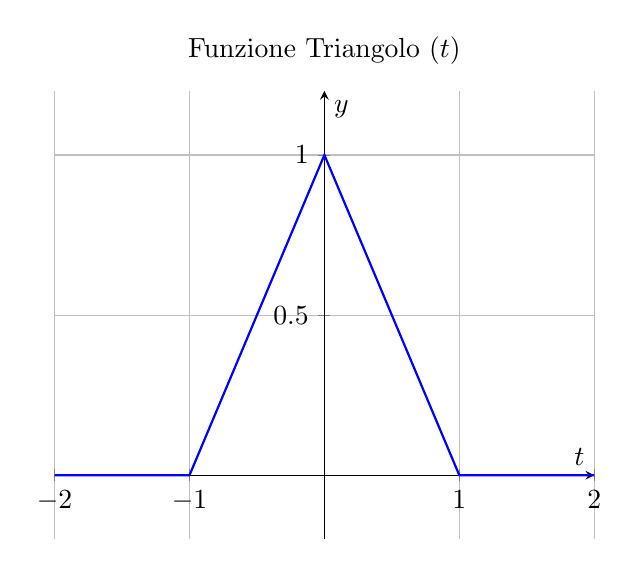
\begin{tikzpicture}
            \begin{axis}[
                axis lines=middle,
                xlabel=$t$,
                ylabel={$y$},
                title={Funzione Triangolo $\tri(t)$},
                xmin=-2, xmax=2,
                ymin=-0.2, ymax=1.2,
                enlargelimits=false,
                grid=major,
            ]
            \addplot[blue, thick] coordinates {(-2,0) (-1,0) (0,1) (1,0) (2,0)};
            \end{axis}
        \end{tikzpicture}
    \end{figure}

\end{itemize}
